The synthetic nervous system controller is developed with a <insert name here>
neuron model. The neurons are modeled with a resting potential of -60 mV and a
maximum potential of -40 mV for a range of 20 mV.

% TODO(buckbaskin): make the capitalization of the networks consistent

\bbs{Key Neurons and Synapses}

% 1 (go through images first)
% TODO(buckbaskin): Define important synapses in model
Transfer, Inversion, Inverted Transfer, etc. 

\bbs{Sensor Fusion}

The Sensor Fusion neuron network performs essentially the same function as the
sensor fusion network in the prototype controller. In this case, 3 neurons
represent the 3 sensor inputs available in a joint: position (``Theta"),
extension muscle pressure (``Ext Pres") and flexion muscle pressure
(``Flx Pres"). The outputs for the network are the estimates for current 
position, velocity and acceleration.

\bbss{Velocity Fusion Network Components}

\bbsss{Differentiator Network}

% 2
% TODO(buckbaskin): talk about differentiator network
The velocity network is based on the Differentiator Network presented in 
\cite{NickFunctionalSubnetwork}.

% 3
% TODO(buckbaskin): Figure of differentiator network

\bbss{Velocity Fusion Network}

The velocity network is based on the Differentiator network. 
The one major change from the network,
as presented, is the inclusion of a second $U_{post}$ neuron to represent the
negative derivative of the position (negative velocity).

% 4
% TODO(buckbaskin): Figure of my velocity network

% TODO(buckbaskin): make sure my inhibitory and excitatory synapses are visualized properly

This represents
a common pattern used across the network where two neurons are used to represent
a single value. One neuron represents positive levels of the variable and is 
at or below resting potential when the value is negative. The other neuron is
above resting potential for negative values and is at or below resting potential
when the value is positive. 

The motivation for increasing the complexity of the
network (often making it more than twice as complicated) is to increase the
effective range of values that the neuron can represent at the same fidelity and
to increase the accuracy of zero. When a single neuron represents positive and
negative values of equal magnitude, the value of 0 is represented at 50 mV; 
however, after passing through a signal transfer neuron this value is often
slightly higher, up to 52 mV. This means that comparing the two neurons (the
original neuron and the signal transfer) yields a slightly positive error
instead of near zero error.

\bbss{Acceleration Fusion Network Components}

\bbsss{Absolute Value Network}

Within the acceleration fusion network, the absolute value of the position is
used. This is calculated by first splitting the position into its two neuron
representation. From there, the sum of the two neurons is used as the absolute
value. This takes advantage of the definition of each side of the two neuron
representation falling below resting potential when the other neuron is active.
This means the signal transfer synapse from the below zero neuron will have no
effect.

% 5
% TODO(buckbaskin): Figure of my absolute value network

\bbsss{Integration Network}

The integration network used throughout the neuron controller is based heavily
on the Integrator Network in \cite{NickFunctionalSubnetwork}. Two neurons are
designed to mutually inhibit each other so that the combined pair hold their
values. Individual neurons can be treated as a leaky integrator; however, their
voltage tails off over time if there is no maintenance current. The integration
network itself is tuned by changing the time constant of the component neurons
to adjust how much the voltage of the integrator network changes for an input
current.

\bbsss{Convert Torque to Pressure}

% 6
% TODO(buckbaskin): talk about how this approximation came about through simulation
Linearized approximation to help with neurons

% TODO(buckbaskin): regenerate the PressureTorque figure with axis labels
\begin{figure}[h!]
\centering
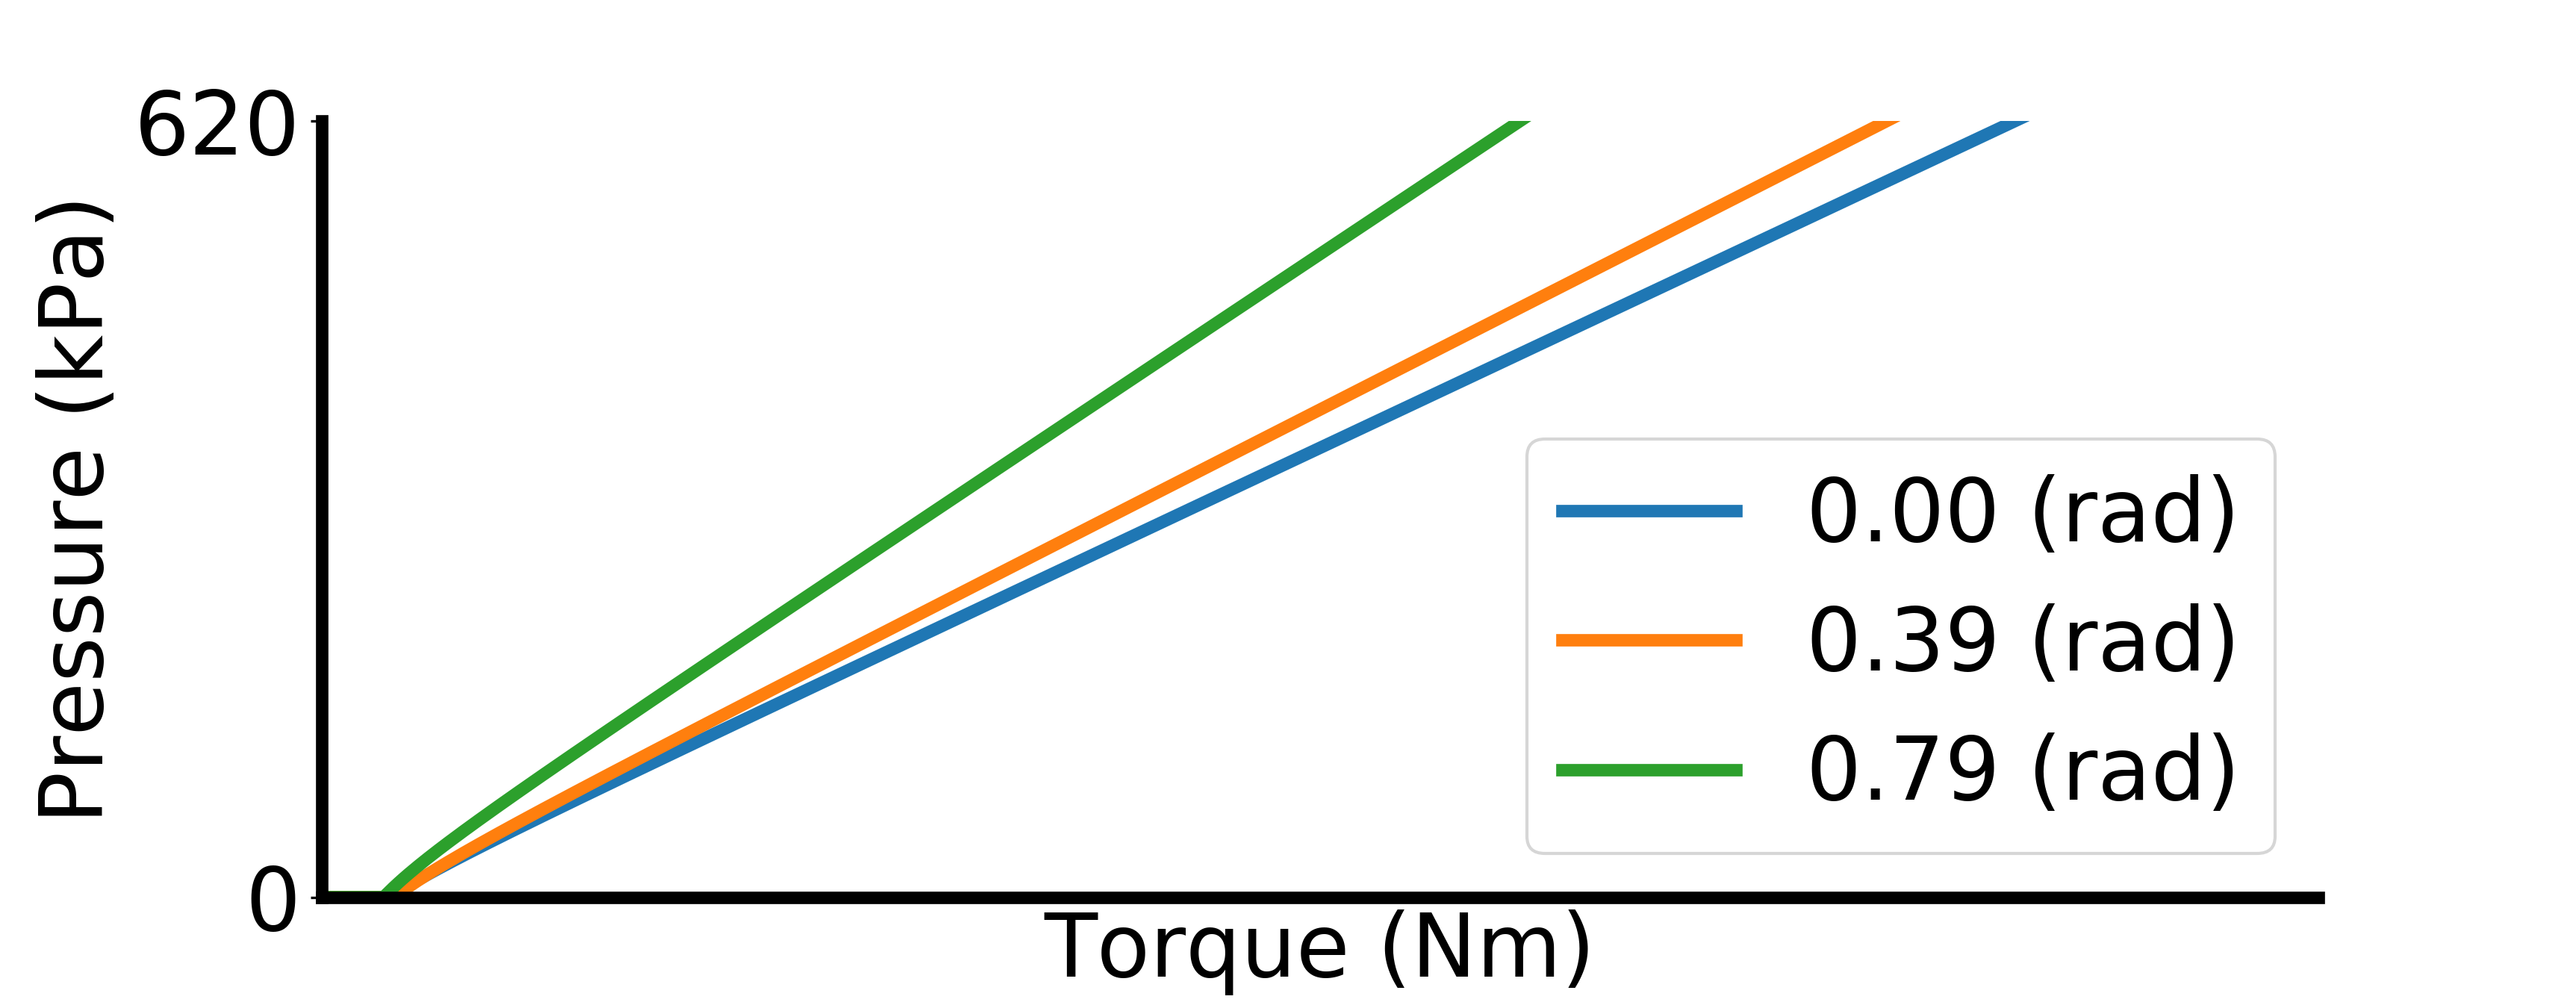
\includegraphics[width=5in]{neuron_design/FigPressureTorque}
\caption{Torque/Pressure relation observed in simulation}
\label{fig:PressureTorque}
\end{figure}

\bbsss{Pressure Estimation Loop}

Within the Acceleration Network, there is a feedback loop that is used to 
estimate the torque applied by a given pressure. First, the loop ``initializes"
with an extension torque guess from the integrator. Second, the extension
torque is converted into extension pressure. Third, the estimated extension
pressure is compared with the sensed pressure. If there is an delta between the
two, the extension torque guess is modified in turn and the cycle repeats.

% 7
% TODO(buckbaskin): Figure of pressure loops

This architecture is mirrored for flexion torque.

\bbss{Torque to Acceleration Network}

% 8
% TODO(buckbaskin): talk about T2A

\bbss{Acceleration Fusion Network}

The acceleration fusion network is a combination of an integrator, absolute
value network, the pressure estimation loop and a torque to acceleration
network. In total, the network uses a combination of smaller networks to
estimate the torque applied from sensed pressure and then combine the extension
and flexion torques together to get a net torque and acceleration.

\section{Optimizing Torque Control}

% 9
I/O summarizing, goals
position, velocity, desired position -> torque

\subsection{Small Networks}

% 10

\subsection{Mid Networks}

% 11

\subsection{Entire Network}

% 12

\section{Torque to Pressure}

% 13
I/O summarizing, goals
convert desired torque pressure in neurons

\subsection{Small Networks}

% 14

\subsection{Mid Networks}

% 15

\subsection{Entire Network}

% 16

\section{System Modeling}

% 17
I/O summarizing, goals
Parameter weight updates

\subsection{Small Networks}

% 18

\subsection{Mid Networks}

% 19

\subsection{Entire Network}

% 20